\documentclass[a4paper,10pt]{article}
\usepackage{amsthm}
\usepackage{amssymb}
\usepackage{enumerate}
\usepackage{amsmath}
\usepackage{extarrows}
\usepackage{mathrsfs}
\usepackage[margin=1in]{geometry}
\usepackage{graphicx}
\usepackage[UseMSWordMultipleLineSpacing,MSWordLineSpacingMultiple=1.5]{zhlineskip}
\usepackage{lipsum}
\usepackage{ctex}
\newtheorem{definition}{定义}[subsection]
\newtheorem{theorem}{定理}[section]
\newtheorem{example}{例子}
\newtheorem{remark}{评论}
\newtheorem{corollary}{推论}
\newtheorem{proposition}{命题}
\newtheorem{problem}{问题}
\bibliographystyle{plain}
\begin{document}
\title{极值点偏移}
\author{lin150117}
\maketitle
\tableofcontents
\noindent
\section{绪论}
导数作为与高等数学最贴近的数学高考方向,具有一定的难度,需要读者对函数的相关知识有深刻的理解,理解“变化率”等概念。

导数主要考察两个部分:一个是“如何去证明题目”,即相关导数方法,另一个是考察代数变形能力,函数构建能力,即思想方法的考察。其中后者是做任何代数题目所必须的,可以说几乎所有的代数题目的关键就是在能不能通过代数变形得到一些什么,能不能构造一个很好的函数。后者需要经验的积累,笔者建议平时要多关注答案为什么这样变形,这样变形的有什么好处。事实上,通常的变形就只有几种类型,其原因和动机也是很容易揣测的,例如 $ |X|  $,看到绝对值或者根号想着平方绝对不是一件坏事,这在向量题目里颇有体现,平方向量通常会让你豁然开朗。

在导数中也是一样,很明显的例子是涉及L'Hospital(洛必达)法则时,当我们要证明一个分式是形如 $ \dfrac{\ln x}{x-1} $,在 $ x\rightarrow1  $ 时分式上下均趋于0,这是我们不想看到的,于是我们会考虑将 $ x-1  $ 乘到右边去(一般我们是去证明不等式)。这也说明等式两边\textbf{乘上或除以一个数}(尤其是乘)会对结果产生非常不同的影响,上面就是一个很好的例子。

分式的处理是导数的非常关键的考察方面。在初等数学中,唯一难求的导数就是分式的导数。上面提到的乘上或除以一个数是一种考虑方法。对分式的变形也是很重要的, $ \dfrac{x+a}{x+b }=\dfrac{a-b}{b+x}+1 $,等式两边求导的难度显然的不同,简单的变形也可能产生很不一样的效果。 当然我们还可以考虑\textbf{取倒数}的方法,这在我们研究数列问题的时候经常用到。

当然取倒数的方法更多还是用在\textbf{换元}上。换元是一个非常重要的技巧,常见的换元手法有:线性代换(例如 $ t=x+y,u=y+z,w=x+z $ 的代换),三角换元,倒数代换(在有很多分式的情况下,用 $ \dfrac{1}{x} $ 的代换往往有奇效,举个简单的例子, $ \dfrac{x }{1+x} $ 用 $ t=\dfrac{1 }{x} $ 代换后得到 $ \dfrac{1}{1+t} $(就是把x除到分母里),两者的求导就有区别了,这在二次以上的式子里会很明显)以及\textbf{整体代换}(常见的有 $ e^x,\ln x,x+\dfrac{1}{x} $ 等等)

我们不得不承认这里的变形和换元都非常简单,甚至我们做题的时候下意识就是会把他们进行这样那样的操作,但是写下来和在脑子里想有很大的区别,笔者警告诸位用脑子想是一个非常愚蠢的事情。我们不应该把小聪明花在这样的地方,因此该写的都尽量写。你会发现,当你进行这样简单的变形后,整个题目就会变的简单不少,这也是导数的神奇之处。

其他的变形限于笔者水平不能一一赘述,还请读者在做题时多关注一下!

但本文的重点不是在于变形,尽管我们可以在接下来的题目中经常看见变形,变形本身就是无法避免的。本文的主要目的是介绍“极值点偏移”以及相关拓展问题,主要想让读者了解“如何去证明一道导数题”的相关思想方法。
\section{极值点偏移问题}
下面这道题是极值点偏移问题的典型例子:

\begin{example}
    已知函数 $ f(x)=x\cdot e^{-x}(x\in\mathbb{R }) $. 如果 $ x_1\not=x_2  $,且 $ f(x_1)=f(x_2) $,证明: $ x_1+x_2>2 $   
\end{example}

一种偏技巧的例子是这样的:

\begin{proof}
    设 $ t=\dfrac{x_1 }{x_2 } $,由题设知 $ \dfrac{x_1 }{x_2 }=\dfrac{e^{x_1}}{e^{x_2}}=e^{x_1-x_2} $. 故 $ \ln t=x_1-x_2=tx_2-x_2\Rightarrow x_2=\dfrac{\ln t}{1-t},x_1=\dfrac{t\ln t }{1-t}\Rightarrow x_1+x_2=\dfrac{(1+t)\ln t  }{1-t} $,只需证明 $ \dfrac{(1+t)\ln t  }{1-t}>2 $.  
\end{proof}

\begin{remark}
    此证明是一个偏代数的证明,其主要考察学生代数变形和换元的能力。值得注意的是, $ t=\frac{x_1 }{x_2 } $ 的换元确实常见,但是一般用于极为对称的情况,在这里的运用笔者也没有见过,而且这里的方法有点类似“你也不知道能不能做,反正试一试”的态度。尝试的确是可以的,但还是要从经验的角度考虑。像这里我们也可以知道一些偏简单的分式方程采用换元也是可以做的,但并不是最普适的方法。

    最后的证明我们要注意变形,即把 $ 1-t  $ 移到右边后再求导。
\end{remark}

\begin{proof}
    由题意可知, $ f(x) $ 在 $ (-\infty,1) $上单调递增,在 $ (1,+\infty ) $ 上单调递减 $ (\star) $  。不妨 $ 0<x_1<1<x_2$,检验 $ f(x)<f(2-x) $ 在 $ x<1 $ 时成立(为什么)于是 $ f(x_2)=f(x_1)<f(2-x_1) $,由单调性知 $ x_2>2-x_1 $,即 $ x_2+x_1>2 $.   
\end{proof}

\begin{remark}
    这个证明就显得自然得多了。那么有这么几点要注意:
    \begin{enumerate}[$ (1) $]
        \item 我们肯定是希望得到一个单变元问题,于是我们考虑把一个元移到右边去(变形\textbf{key})。
        \item 考虑单变元问题是肯定的,因为从逻辑上考虑,如果我们确定了 $ x_1 $,在几何上很容易看出 $ x_2  $ 已经唯一确定,因此 $ x_2  $ 是不必须的。
        \item 移到右边去后的考量就是能不能有某种单调性。于是我们考查一下 $ f(x)  $ 的单调性,要知道\textbf{单调性是产生导数内不等式的方法之一}。如何考虑则是经验上的问题,如果我们已经发现 $ (\star) $ 的事实,那么我们就可以直接考虑比较 $ f(2-x_2) $ 与 $ f(x_1) $,时刻保持对 $ f(x_1)=f(x_2) $ 的警惕。
        \item 我们也可以从几何的视角来观察这个问题:
        \begin{figure}[htp]
            \centering
            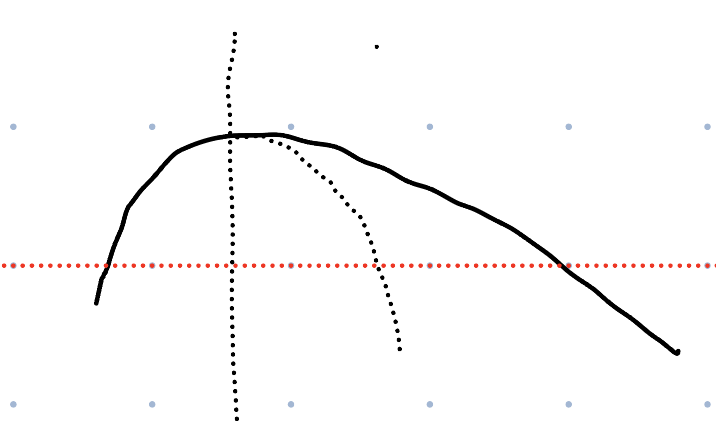
\includegraphics[scale=0.5]{picture1.png}
        \end{figure}

        两者之和不外乎中点上的问题。当然我们这里不考察中点,而是考察对称。这也是一种思想:不去看为什么不等号成立,而去看不等号的极限在哪里。那么我们这里就考虑 $ x_1  $ 这边的点关于 $ x=1  $ 的对称,那么如果结果如上图所示,红线部分很直观的阐述了 $ x_1+x_2>2 $。那么这也就是为什么这个方法产生的原因之一了。我们其实想去描述这样子的现象。很多分析上的问题都有几何上的解释,但是我们要去做的就是利用导数和单调性确定大小关系和变化率。 
    \end{enumerate}
\end{remark}

那么我们从上面的第三点出发给出一个一般的情形。
\begin{problem}
    对一个函数 $ f(x)  $,如果它差不多长成下图或上图这样子,即分段单调且极值点偏移,那么若 $ f(x_1)=f(x_2) $,则 $ x_1+x_2 $ 与极值点 $ x  $ 轴坐标的两倍有某种数量关系。  
\end{problem}
\begin{figure}[htbp]
    \centering
    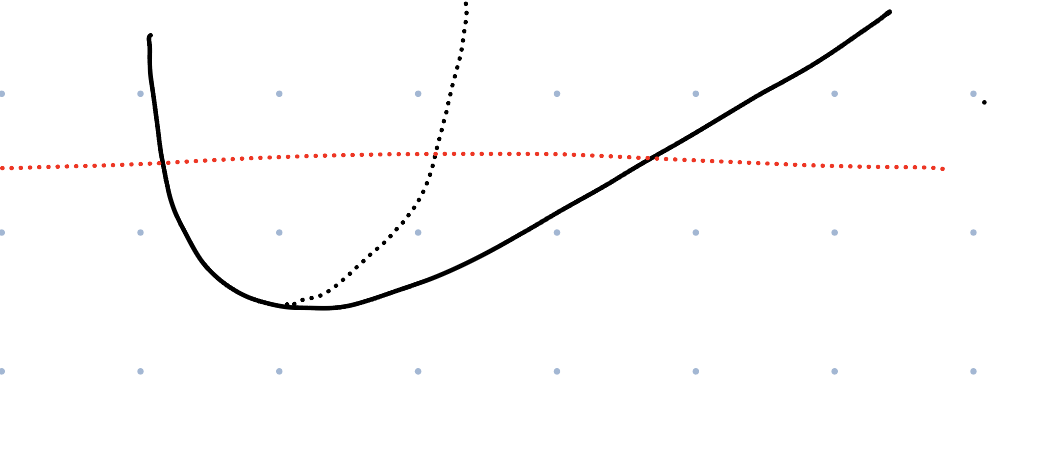
\includegraphics[scale=0.5]{图片1.png}
\end{figure}

那么这种题的解法就是比如:为证明 $ x_1+x_2>2k $ ($ k $为常数),考虑 $ x_1>2k-x_2 $,由函数单调性可知只需证明 $ f(x_1)>f(2k-x_2) $(首先要确定 $ x_1,k  $ 和 $ x_2 $的大小关系。后面就是求导问题。 

当然,从几何的角度来看,我们其实可以归纳出另外一种导数的做法:就以问题里的图为例,其实把左边对称到右边后,我们想要描述这样子的图形,或者说证明 $ x_1+x_2>2k  $,只需证明左边函数的变化率比右边大即可,即 $ |f'(x_1)|>|f'(2-x_1)| $。这可能是另外一种考虑的方法,即考虑导数大小而不考虑原函数大小,导数往往会比原函数简单。这一点也是为什么极值点偏移单独来讲的缘故,因为函数性质非常丰富,有时读者做题时必须要考虑这些事。

然而,不得不承认的是,所谓“几何的直观”不过是愚人的小把戏而已。前人已经我们踩过了太多坑,我们不能再沉迷于邪淫的技巧之中而忽视了那些本质而抽象的东西---思想和方法。这在接下来拓展的习题里也有体现。
\section{举一反三}
\begin{example}[镇海中学2024高考模拟]
    定义 $ \phi(y)=\dfrac{2\sqrt{2}|y''|}{|1+y'|^3} $ 为 $ y=f(x) $ 的“柯西曲率”。已知 $ f(x)=x\ln x-2x $ 上存在两点 $ P(x_1,f(x_1)),Q(x_2,f(x_2)) $ 的“柯西曲率”相同。求 $ \sqrt[3]{x_1}+\sqrt[3]{x_2} $ 的取值。
\end{example}
\begin{remark}
    那么这一道题呢和常规的极值点偏移问题的区别就是1、两数之和变成了开立方后之和;2、由证明不等式变成了证明取值。但是它的本质是不变的,开立方并没有对我们(非几何)的证明方法产生任何影响,换言之,我们可以直接进行 $ t_i=\sqrt[3]{x_i } $ 的换元。事实上,不管我们要求 $ x_1x_2,x_1-x_2 $ 或者 $ x_1/x_2 $ 等等,都可以变形或换元。
    
    但是取值对我们这道题产生了一定的影响,但是范围方面的问题,我们有两种处理手段:一是用变元(最好为一个)表示出要求范围的量;二是\textbf{先猜后证}。对于这样“连续”的问题,一般都是在极端情况下产生,那么我们猜出答案,只要证明两个不等式就好了。
\end{remark}

\begin{example}[\cite{ZSJC202103016}]
    已知函数 $ f(x)=x^2+x+2\ln x  $,若 $ f(x_1)+f(x_2)=4  $,求证: $ x_1+x_2 \geq 2 $. 
\end{example}
\begin{remark}
    这里的问题则是条件的变化。然而,如果按照我们的证明方法,先变不等式,利用单调性变成求解单变元导数不等式。本题并没有什么本质上的不同。
\end{remark}
极值点偏移问题其实就是我们解决条件下二元不等式的方法。其基本策略就是移项变化不等式,利用单调性变成函数间的不等式,利用条件变成单一变量的导数不等式。根本的想法就是转化成一元不等式来处理。

另外,拉格朗日乘数法则是更一般情形下的处理方法(不能用但可以用来猜答案)\cite{FZSX202307015}
\begin{theorem}[Lagrange]
    给定二元函数 $ z=f(x,y)  $ 在条件 $ \phi(x,y)=0 $ 下,设 $ F(x,y,\lambda)=f(x,y)+\lambda\phi(x,y)$,则当 $ f(x,y) $ 取得极值点时, $ F(x,y,\lambda) $ 分别以 $ x,y,\lambda  $ 为主元的导数均为零。即 $ F'(x,y,\lambda)=0 $ 或者说
    \begin{equation}
        \left\{
            \begin{aligned}
                {}&\dfrac{\mathrm{d}F(x,y,\lambda)}{\mathrm{d}x}=0\\
                {}&\dfrac{\mathrm{d}F(x,y,\lambda)}{\mathrm{d}y}=0\\
                {}&\dfrac{\mathrm{d}F(x,y,\lambda)}{\mathrm{d}\lambda}=\phi(x,y)=0
            \end{aligned}
        \right.
    \end{equation}   
\end{theorem}
\bibliography{article}
\end{document}